\documentclass[review,sigconf]{acmart}

%\usepackage[table]{xcolor}
\usepackage{xcolor}
\usepackage{booktabs} % For formal tables
\usepackage{numprint}
\usepackage{xspace}
%\usepackage{cite}
\usepackage{amsmath,amssymb,amsfonts}
\usepackage{algorithmic}
\usepackage{graphicx}
\usepackage{color}
\usepackage{textcomp}
\usepackage[normalem]{ulem}
\usepackage{soul}
\usepackage{multirow}
\usepackage{dblfloatfix}


%\usepackage[table,xcdraw]{xcolor}
%\usepackage[table]{xcolor}
%--
\newcommand{\ignore}[1]{ } % ignore blocks of text
\newcommand{\maketiny}[1]{{\tiny G: #1}} % ignore blocks of text
\newcommand{\ganesh}[1]{\todo[inline,size=\small, color=purple!40]{G: #1}}

\newcommand{\parlot}{\textsc{ParLoT}\xspace}
\newcommand{\pin}{\textsc{PIN}\xspace}
\newcommand{\callgrind}{\textsc{Callgrind}\xspace}

%--\newcommand{\circleRtool}{circleRtool\circledR\xspace}

%%% Local Variables:
%%% mode: latex
%%% eval: (flyspell-mode 1)
%%% TeX-master: "root.tex"
%%% End:

%--



% Copyright
%\setcopyright{none}
%\setcopyright{acmcopyright}
%\setcopyright{acmlicensed}
%\setcopyright{rightsretained}
%\setcopyright{usgov}
%\setcopyright{usgovmixed}
%\setcopyright{cagov}
%\setcopyright{cagovmixed}


\begin{document}

\title{ DiffTrace: Efficient Whole-Program Trace Analysis and Diffing}


\author{Saeed Taheri}
\email{staheri@cs.utah.edu}
\affiliation{%
  \institution{University of Utah}
  \city{Salt Lake City}
  \state{Utah}
  \country{United States}
}

\author{Ian Briggs}
\email{ianbriggsutah@gmail.com}
\affiliation{%
  \institution{University of Utah}
  \city{Salt Lake City}
  \state{Utah}
  \country{United States}
}

\author{Martin Burtscher}
\email{burtscher@cs.txstate.edu}
\affiliation{%
  \institution{Texas State University}
  \city{San Marcos}
  \state{Texas}
  \country{U.S.A.}
}

\author{Ganesh Gopalakrishnan}
\email{ganesh@cs.utah.edu}
\affiliation{%
  \institution{University of Utah}
  \city{Salt Lake City}
  \state{Utah}
  \country{U.S.A.}
}





%\renewcommand{\shortauthors}{S. Taheri et al.}

\begin{abstract}
\label{abs}
The need for efficient tracing to gain insight into
HPC application executions is growing. 
%
Unfortunately, available tools either do not produce traces with enough details,
or incur huge overheads.
%
An efficient  tracing method that overcomes the trade off
between maximum information and minimum overhead
is needed for today's HPC application developers.
% 

In this paper, we present \parlot, a tool that provides several key
features (1)~It dynamically instruments the binary without source-code modification or recompilation.
%
(2)~It employs a set of highly efficient trace compression methods that reduces the trace volume gathered at runtime dramatically, thus making tracing cheaper.
%
(3)~It supports program analysis and debugging by
including caller/callee
relations, call frequencies, and a linear trace of entire executions
at the granularity the user opts for.
%
This paper establishes that comparable capabilities are 
unavailable by evaluating the best alternative tracing options
on runs up to 1,024 cores on the NAS parallel benchmarks on the
Comet supercomputer.
%
Our experiments show that \parlot can produce whole-program function 
call traces with average of 56 kB/s required bandwidth while 
slowing down applications by 2.7x on average. 

\end{abstract}

\keywords{diffing, tracing, debugging}

\maketitle


\section{Introduction}
\label{sec:intro}
Debugging high-performance computing code
remains a challenge at all levels of scale.
%
Conventional HPC debuggers~\cite{allinea-ddt,roguewave,others}
excel at many tasks such as examining the execution
state of a complex simulation in detail
and allowing the developer to re-execute
the program close to the point of failure.
%
However, they do not provide a good understanding
of why a program version that worked earlier
failed upon upgrade or feature addition.
%
Innovative solutions are needed to highlight the
salient differences between two executions in a manner
that makes debugging easier as well as more systematic.
%
A recent study conducted under the auspices of the
DOE~\cite{DBLP:journals/corr/GopalakrishnanH17}
provides a comprehensive survey
of existing debugging tools.
%
It classifies them under
four software organizations (serial, multithreaded,
multi-process, and hybrid), six
method types (formal methods, static analysis, dynamic
analysis, nondeterminism control, anomaly detection,
and parallel debugging), and lists a total of 30 specific
tools.
%
Despite this abundance of activity and tools, many
significant problems remain to be solved before debugging
{\em can be approached by the HPC community as a collaborative
activity} so that HPC developers can share their solutions
and extend a common framework.

Almost all debugging approaches seek to find outliers (``unexpected
executions'') amongst thousands of running processes and threads.
%
The approach taken by most existing tools is to
look for symptoms in a specific bug-class that they cover.
%
Unfortunately,
this approach calls for a programmer having a good guess of what
the underlying problem might be,
and to then pick the right set of tools to deploy.
%
If the guess is wrong, the programmer has no choice but to
refine their guess
and look for bugs in another class,
re-executing the application and hoping for
better luck with another tool.
%
This iterative loop of re-execution followed by applying a
best-guess tool for the suspected bug class can potentially consume
large amounts of execution cycles and wastes an
expert developer's time.
%
More glaring is the fact that these tools must recreate the
execution traces yet again: they do not have means to hand off
these traces to another tool or cooperate in symbiotic ways.



We cannot collect all relevant pieces of information
necessary to detect all possible bug classes such as
resource leaks, deadlocks, and data races.
%
Each such bug requires its own attributes to be kept.
%
Also, debugging is not fully automatable (it is
an undecidable problem in general) and must involve human thinking:
at least to reconcile what is observed against the deeper application-level semantics.
%
However, (1)~we believe that it is still possible to collect one common set
of data and use it to make an initial triage in such
a way that it can guide a later, deeper debugging phase to locate
which of the finer bug gradations (e.g., resource leaks or races) brought
the application down.
%
Also, (2)~we believe that it is possible to engage the human {\em with respect
to understanding structured presentations of information}---as opposed to a general
disorienting bug situation.


Our DiffTrace framework addresses both issues.
%
The common set of data it uses is a {\em whole program
function call trace} collected per process/thread.
%
DiffTrace relies on
novel ways to diff a normal trace and a fault-laden trace to guide the
debugging engineer closer to the bug.
%
While our work has not (yet) addressed situations in
which millions of threads and thousands of processes run
for days before they produce an error,
we strongly believe that we can get there
once we understand the pros and cons of our initial
implementation of the DiffTrace tool, which are described in this paper.
%
The second issue is handled in DiffTrace by offering a novel
collection of modalities for understanding program execution diffs.
%
We now elaborate on these points by addressing the following three problems.



\paragraph{Problem 1 -- Collecting Whole-Program Heterogeneous Function-Call Traces
Efficiently\/} Not only must we have the ability
to record function calls and returns at one
API such as MPI, increasingly we must collect calls/returns at multiple
interfaces (e.g., OpenMP, PThreads, and even inner levels such as TCP).
%
The growing use of heterogeneous parallelization necessitates that we 
understand MPI and OpenMP activities (for example) to locate cross-API
bugs that are often missed by other tools.
%
Sometimes, these APIs contain the actual error (as opposed to the user code), and it would be attractive to have this debugging ability.


{\em Solution to Problem 1:\/}
In DiffTrace, we choose PIN-based whole program binary tracing, with
tracing filters that allow the designer to collect a suitable mixture of API
calls/returns.
%
We realize this facility using
ParLoT, a tool designed by us and published earlier~\cite{parlot-paper}.
%
In our research, we have thus far demonstrated the advantage of
ParLoT with respect to collecting both MPI and OpenMP traces
from a {\em single run of a hybrid MPI/OpenMP program}.
%
We demonstrate that, from this single type of trace, it is possible
to pick out MPI-level bugs and/or OpenMP-level bugs.
%
While whole-program tracing
may sound extremely computation and storage intensive, ParLoT employs
lightweight on-the-fly compression techniques to keep these overheads low.
%
It achieves compression ratios exceeding 16,000~\cite{parlot-paper},
thus making this approach practical, demanding
only a few kilobytes per second per core of bandwidth.


\paragraph{Problem 2 -- Need to Generalize Techniques for Outlier Detection\/}
Given that outlier detection is central to debugging,
it is important to use efficient representations of the traces
to be able to systematically compute
{\em distances} between them without
involving human reasoning.
%
The representation must also be versatile enough to
be able to ``diff'' the traces
with respect to {\em an extensible number of vantage points}.
%
These vantage points could be diffing with respect to process-level activities,
thread-level activities, a combination thereof,
or even finite sequences of process/thread calls (say, to locate {\em changes}
in caller/callee relationships).


{\em Solution to Problem 2:\/}
DiffTrace employs {\em concept lattices} to amalgamate the collected traces.
%
Concept lattices have previously been employed in HPC to perform structural
clustering of process behaviors~\cite{weber-cl} to present performance data more
meaningfully to users.
%
The authors of that paper use the notion of {\em Jaccard distances}
to cluster performance results that are closely related to process structures
(determined based on caller/callee relationships).
%
In DiffTrace, we employ incremental algorithms for building and maintaining
concept lattices from the ParLoT-collected traces.
%
In addition to Jaccard distances, in our work we also perform hierarchical
clustering of traces and provide a tunable threshold for outlier detection.
%
We believe that these uses of concept lattices and refinement approaches
for outlier detection are new in HPC debugging.


\paragraph{Problem 3 -- Loop Summarization\/}
Most programs spend most of their time in loops.
%
Therefore, it is important to employ state-of-the-art algorithms for
loop extraction from execution traces.
%
It is also important
to be able to diff two executions with respect to changes in their looping behaviors.
%
In our experience, presenting such changes using good visual metaphors
tends to immediately highlight many bug types.


{\em Solution to Problem 3:\/}
DiffTrace utilizes the rigorous notion of Nested Loop Representations (NLRs) for
extracting loops.
%
Each repetitive loop structure is given an identifier, and nested loops are
expressed as repetitions of this identifier exponentiated (as with regular
expressions).
%
This approach to summarizing loops can help manifest
bugs where the program does not hang or crash but nevertheless
runs differently in a manner that informs the developer engaged in debugging.

{\bf Contributions and Organization\/}:
\S\ref{sec:overview} illustrates the contributions of this paper on a simple example.
%
\S\ref{sec:algo} presents the algorithms underlying DiffTrace in more detail.
%
\S\ref{sec:ilcs-case-study} shows a medium-sized case study involving MPI and OpenMP.
%
\S\ref{sec:experimental} summaries the experimental methodology before presenting results for LULESH~\cite{lulesh}, a DOE common mini app.
%
\S\ref{sec:related} summarizes selected related works.
%
\S\ref{sec:discussion} concludes the paper with a discussion.

% 
% \Noindent To summarize, the key contributions of this paper are the following
% \begin{itemize}
% \item A method to organize function call traces collected from processes and
%       threads into concept lattices, and a method to
%       detect loops from dynamic traces (Section~\ref{sec3}).
% 
% \item Details of the algorithms employed in DiffTrace (Section~\ref{sec4}).
% 
% \item Experimental studies on a heterogeneous program called
%       Iterated Local Champion Search (ILCS, Section~\ref{sec5}).
% 
% \item Strengths and limitations of DiffTrace, plans for future work (Section~\ref{sec6}).
% \end{itemize}
% 


% 
% \hl{[[Ganesh and Saeed have written some text before for the intro which is available in v0/intro.tex (also available but commented in current file). Current version is based on our discussion on May 8th]]}
% 
% \begin{itemize}
% 	\item Importance of whole program diffing: understand changes, debug (DOE REPORT \cite{hpcdoe})
% 	\item Efficient tracing supports selective monitoring at multiple levels
% 	\begin{itemize}
% 		\item Bugs not there at a predictable API level
% 		\item Prior work (ParLoT) supports whole program tr.
% 	\end{itemize}
% 	\item Dissimilarity is important to know: bugs, changes during porting, ...
% 	\item Key enablers of meaningful diffing:
% 	\begin{itemize}
% 		\item Formal concepts (novel contrib to debugging)
% 		\item Loop detection (loop diffing can help)
% 	\end{itemize}
% 	\item Importance, given the growing heterogeneity
% \end{itemize}
% 
% 
% %When a new version of an HPC software system is created, logical errors often get introduced.
% %
% %To maintain productivity, designers need effective and efficient methods to locate these errors.
% %
% %Given the increasing use of hybrid (MPI + X) codes and library functions, errors may be introduced through a usage contract violation at multiple interfaces.
% %
% %Therefore, tools that can record activities at all involved APIs are necessary.
% %
% %Designers find most of these bugs manually, and the efficacy of a debugging tool is often measured by how well it can highlight the salient differences between the executions of two versions of software.
% %
% %Given the huge number of things that could be different -- individual iterative patterns of function calls, groups of functions calls, or even specific instruction types (e.g., non-vectorized versus vectorized floating-point dot vector loops) -- designers cannot afford to rerun the application many times to collect each facet of behavior separately.
% %
% %These issues are well summarized in many recent studies \cite{hpcdoe}
% 
% 
% %One of the major challenges of HPC debugging is the huge diversity of applications, which encompass domains such as computational chemistry, molecular dynamics, and climate simulation.
% %
% %In addition, there are many types of possible “bugs” or, more precisely, errors. An \textbf{error} may be a deadlock or a resource leak. These errors may be caused by different \textbf{faults}: an unexpected message reordering rule (for a deadlock) or a forgotten free statement (for a resource leak).
% %
% %There exists a collection of scenarios in which a bug can be introduced: when developing a brand-new application, optimizing an existing application, upscaling an application, porting to a new platform, changing the compiler, or even changing compiler flags.
% %
% %Unlike traditional software, there are hardly any bug-repositories, collection of trace data or debugging-purpose benchmarks in the HPC community.
% %
% %The heterogeneous nature of HPC bugs makes developers come up with their own solutions to resolve specific classes of bugs on specific architectures or platforms that are not usable elsewhere \cite{hpcdoe}.
% 
% % Why we need always on tracing
% %When a failure occurs (e.g., a deadlock or crash) or the application outputs an unexpected result, it is not economic to rerun the application and consume resources to reproduce the failure. Moreover, HPC bugs might not be reproducible due to non-deterministic behavior, which is common in HPC applications. Also, the failure might be caused by a bug present at different APIs, system levels or the network, thus multiple reruns might be needed to locate the bug.
% 
% %ParLOT introduction
% %In previous work \cite{parlot}, we have introduced ParLoT, a tool that efficiently collects whole program function-call traces using dynamic binary instrumentation.
% %
% %ParLOT captures function calls and returns at different levels (e.g., application and library code) and incrementally compress them on-the-fly, resulting in low runtime overhead and low tracing bandwidth, preserving the whole-program dynamic behavior for offline analysis.
% %
% 
% % Post-mortem analysis to obtain understanding about different aspects of the dynamic behavior
% %In the current work, we introduce DiffTrace, a tool-chain for the post-mortem analysis of \textit{ParLoT Traces} (PTs) that supplies developers with information about dynamic behavior of HPC applications at different levels with different granularities towards debugging. 
% %
% %The topology of HPC tasks on both distributed and shared memory often follows a ``symmetric'' flow of control such as SPMD, master/slave, or odd/even where multiple tasks contain \textit{similar} events in their control flow.
% %
% %HPC bugs often manifest themselves as divergence in the control flow of processes compared to what was expected.
% %
% %In other words, HPC bugs violate the rule of ``symmetric'' and ``similar'' control flow of one or more threads/processes in typical HPC applications based on the original topology of the application.
% %
% %We believe that finding the dissimilarities among traces is the essential initial step towards locating the bug and identifying the root cause.
% 
% %Large-scale HPC application execution would result in thousands of PTs due to the execution of thousands of processes and threads.
% %
% %Since HPC applications spend most of their time in an outer main loop, every single PT also may contain sequences of millions of trace entries (i.e., function calls and returns).
% %
% %Finding the bug manifestation (i.e., dissimilarities caused by the bug) among many long PTs is the problem of finding the needle in the haystack.
% 
% %
% %Decompressing PTs collected from long-running large-scale HPC applications for offline analysis produces an overwhelming amount of data. However, missing any piece of collected data may result in losing key information about the application behavior.
% %
% %We propose a variation of the NLR (Nested Loop Recognition) algorithm \cite{Ketterlin-nlr} that takes a sequence of trace entries as input and, by recursively detecting repetitive patterns, re-compresses traces into ``iterative sets'' in a lossless fashion (intra-PT compression).  
% %
% 
% %Analyzing the application execution as a whole (inter-PT compression) is another goal that we are pursuing in this work. 
% %
% %By extracting \textit{attributes} from pre-processed traces, we inject them into a concept hierarchy data structure called Concept Lattice \cite{clbook}.  
% %
% %Concept lattices give us the capability to reduce the search space from thousands of instances to just a few \textit{equivalence classes of traces} by measuring the similarity of traces \cite{Alqadah2011}, making the process of finding the needle in the haystack more feasible.
% %
% %Comparison of the bug-free concept lattice and its equivalent classes with the buggy version of the same application reveals insights about the dynamic behavior of the program and how the bug changed the classes and their members.
% %
% 
% %Fowlkes et al.~\cite{fowlkes83} proposed a method for comparing two hierarchical clusterings by counting the objects that fall into the same or different clusters.
% %
% %Inspired by Fowlkes's approach, we believe that the PTs that fall into different classes before and after the bug are the potential PTs that manifest the bug impact and/or reflect the bug's root cause.
% %
% %These candidate PTs then require deeper \textit{observing} and \textit{diffing} with their corresponding bug-free PTs to see what has been changed when the bug was introduced.
% %
% \hl{**   TODO: 
% Highlights of results obtained as a result of the above thinking should be here. This typically comes before ROADMAP of paper.}
% 
% In summary, this paper makes the following main contributions:
% \begin{itemize}
% \item A tunable tracing and trace-analysis toolchain for HPC application program understanding and debugging
% \item A variation of the NLR algorithm to compress traces in lossless fashion for easier analysis and detecting (broken) loop structures
% \item An FCA-based clustering approach to efficiently classify traces with similar behavior
% \item A tunable ranking mechanism to highlight suspicious trace instances for deeper study
% \item A visualization framework that reflects the points of differences or divergence in a pair of sequences.
% \end{itemize}
% 
% %
% \hl{
% The rest of the paper is as follows:
% 
% - Sec 2: Background
% 
% - Sec 3: Components
% 
% - Sec 4: Case Study: ILCS
% 
% - Sec 5: Related Work
% 
% - Sec 6: Concluding Remarks
% }
%





\section{cl-Trace Components}
\label{sec:components}
\textbf{\hl{IS THIS SECTION NECESSARY?}}

\subsection{General Idea}

Figure \ref{fig.diffTraceOverview} shows a general overview of DiffTrace and its components.

\begin{figure}[t]
\caption{diffTrace Overview}
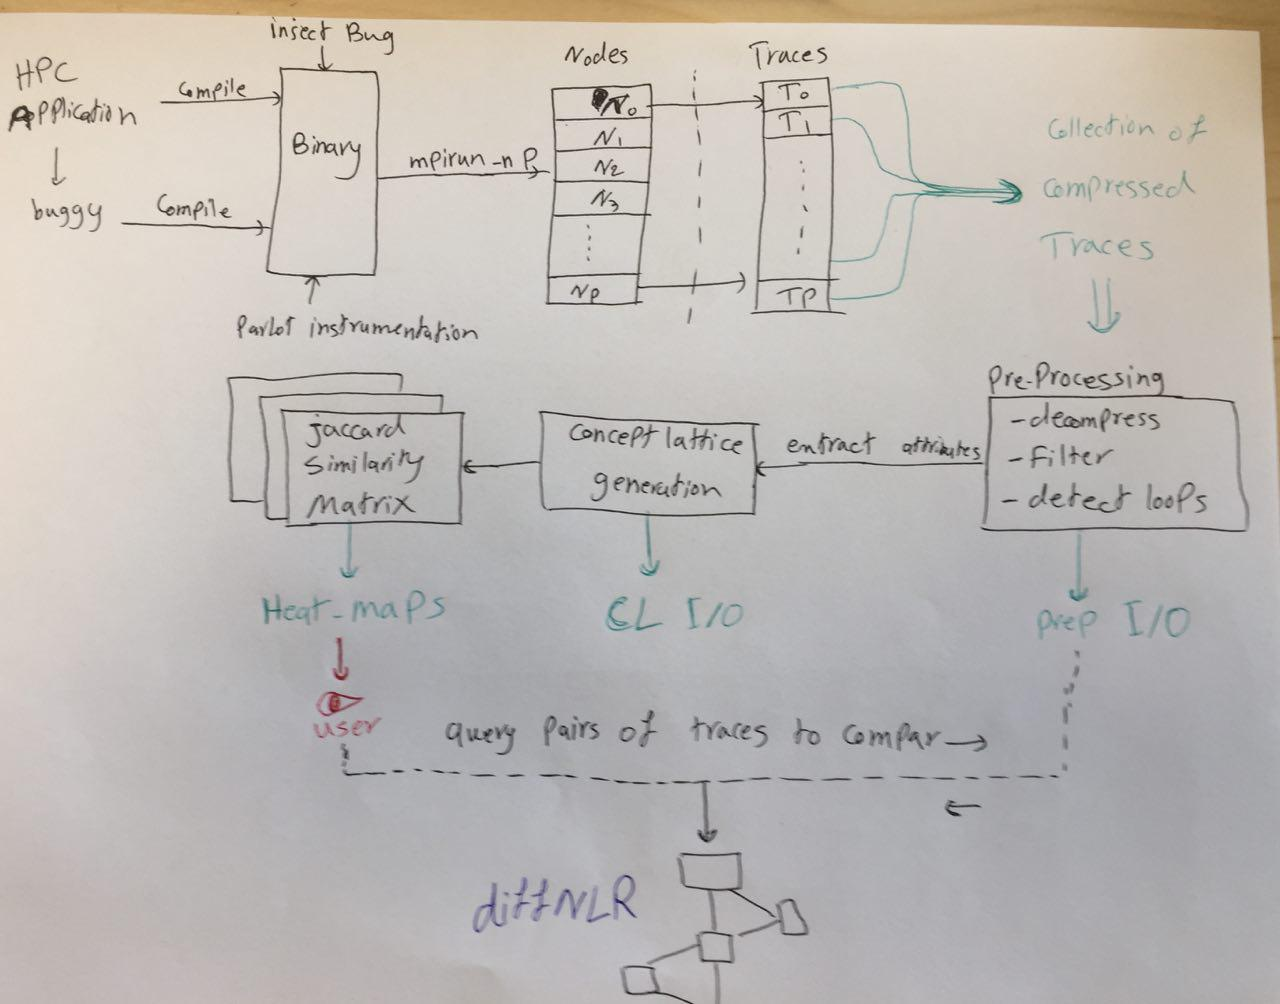
\includegraphics[width=0.45\textwidth]{overviewSketch.jpg}
\label{fig.diffTraceOverview}
\end{figure}


\subsection{Fault Injection??}
\subsection{ParLOT}
How we collect ParLOT traces? Is that necessary?
\subsection{Filter}
Include a table with all filters and their regular expressions
\subsubsection{General Filters}
\begin{itemize}
\item Returns
\item .plt
\item Memory
\item Network
\item Polling
\item String
\item Customize
\item IncludeEverything
\end{itemize}
\subsubsection{Target Filters}
\begin{itemize}
\item MPI\_
\item MPIall
\item MPI\_ Collectives
\item MPI\_ Send/Recv
\item OMPall
\item OMPcritical
\item OMPmutex
\end{itemize}

\subsection{Nested Loop Recognition}
\subsubsection{Background}
\subsubsection{Implementation}


\subsection{Concept Lattice Analysis}
\subsubsection{Background}
\begin{itemize}
\item FCA (formal concept analysis) background and citations
\item FCA applications in all areas
\item FCA applications in Data Mining and Information Retrieval
\item FCA applications in distributed systems (Garg's work)
\item intro to Concept, Object, Attribute and other definitions
\end{itemize}

\subsubsection{Objects/Attributes}


Mapping of Object/Attribute (general) to Trace/Attribute (clTrace)

What do we expect to gain by doing so
\begin{itemize}
\item Single entity represents the whole execution of HPC application (can be used as signature/model in ML)
\item Classifying similar behavior objects(traces)
\item Efficient Incremental CL building makes it scalable 
\item Efficient full pair-wise Jaccard Similarity Matrix extraction 
\end{itemize}
\subsubsection{CL generation}

\begin{itemize}
\item background
\item current approach
\end{itemize}

\subsubsection{Jaccard Similarity Matrix}

\begin{itemize}
\item background
\item LCA
\item Benefits
\end{itemize}


\subsection{diffNLR}
\begin{itemize}
\item motivation
\item diff algorithm
\item visualization
\end{itemize}

\subsection{FP-Trace}


\section{Tool-Chain Design}
\label{sec:design}
Figure \ref{overview} provides a general overview of \parlot 's workflow. Note that the instrumentation takes place dynamically, i.e., right before a new basic block is about to be executed.


\subsection{Tracing Operation}

\parlot is built on top of \pin. In particular, it instructs \pin to instrument every thread launch and termination in the application as well as every function entry and exit. The thread-launch instrumentation code initializes the per-thread tracing variables and opens a file into which the trace data from that thread will be written. The thread-termination code finalizes any ongoing compression, flushes out the remaining buffer entries, and closes the trace file. \parlot assigns every static function in each image (main program and all libraries) a unique unsigned 16-bit ID, which it records in a separate file together with the image and function name. This file later serves to map IDs back to function-name/image pairs.

For every function \emph{entry}, \parlot executes extra code that has access to the thread ID, function ID, and current stack-pointer (SP) value. Based on the SP value, it performs call-stack correction if necessary (see below), adds the new function to a data structure it maintains that holds the call stack (which is separate from the application's runtime stack), and emits the function ID into the trace file via an incremental compression algorithm (see below). All of this is done independently for each thread. Similarly, for every function \emph{exit}, \parlot also executes extra code that has access to the thread ID, function ID, and current SP value. Based on the SP value, it performs call-stack correction if necessary, removes the function from its call-stack data structure, and emits the reserved function ID of zero into the trace file to indicate an exit. As before, this is done via an incremental compression algorithm. We use zero for all exits rather than emitting the function ID and a bit to specify whether it is an entry or exit because using zeros results in more compressible output. After all, this way, half of the values in the trace will be zero.


\subsection{Call-Stack Correction}

To be able to decode the trace, i.e., to correctly associate each exit with the function entry it belongs to, our trace reader maintains an identical call-stack data structure. Unfortunately, and as pointed out in the \pin documentation~\cite{???}, it is not always possible to identify all function exits. For example, in optimized code, a function's instructions may be inlined and interleaved with the caller's instructions, making it sometimes infeasible for \pin to identify the exit. As a consequence, we have to ensure that \parlot works correctly even when \pin misses an exit. This is where the SP values come into play.

During tracing, \parlot not only records the function IDs in its call-stack data structure but also the associated SP values. This enables it to detect missing exits and to correct the call stack accordingly. Whenever a function is entered, it checks if there is at least one entry in the call stack and, if so, whether its SP value is higher than that of the current SP. If it is lower, we must have missed at least one exit since the runtime stack grows downwards (the SP value decreases with every function entry and increases with every exit). If a missing exit is detected in this manner, \parlot pops the top element from its call stack and emits a zero to indicate a function exit. It repeats this procedure until the stack is empty or its top entry has a sufficiently high SP value. The same call-stack correction technique is applied for every function exit whose SP value is inconsistent. Note that the SP values are only used for this purpose and are not included in the emitted trace data.

The result is an internally consistent trace of function entry and exit events, meaning that parsing the trace will yield a correct call stack. This is essential so that the trace can be decoded properly. Moreover, it means that the trace includes exits that truly happened in the application but that were missed by \pin. Note, however, that our call-stack correction is a best-effort approach and may, in rare cases, temporarily not reflect what the application actually did. This can happen for functions that do not create a frame on the runtime stack.


\subsection{Incremental Compression}

\parlot immediately compresses the traced information even before it is written to memory. In other words, it compresses each function ID before the next function ID is known. The conventional approach would be to first record uncompressed function IDs in a buffer and later compress the whole buffer once it fills up. However, this makes the processing time very non-uniform. Whereas almost all function IDs can be recorded very quickly since they just have to be written to the buffer, processing a function ID that happens to fill the buffer takes a long time as it triggers the compression of the entire buffer. This results in sporadic blocking of threads during which time they make no progress towards executing the application code. Initial experiments revealed that such behavior can be detrimental when one thread is polling data from another thread that is currently blocked due to compression. For example, we observed a several order of magnitude increase in entry/exit events of an internal MPI library function when using block-based compression.

To remedy this situation, the compressor must operate incrementally, i.e., each piece of trace data must be compressed when it is generated, without buffering it first, to ensure that there is never a long-latency compression delay. Few existing compression algorithms have been implemented in such a manner because it is more difficult to code up and possibly a little slower. Nevertheless, we managed to implement our algorithm (discussed next) in this way so that each trace event is compressed with similar latency.


\subsection{Compression Algorithm}

We used the CRUSHER framework~\cite{Cluster15, Space16, SC16, DCC18} to automatically synthesize an effective and fast lossless compression algorithm for our traces. CRUSHER is based on a library of data transformations extracted from various compression algorithms. It combines these transformations in all possible ways to generate algorithm candidates, which it then evaluates on a set of training data. We gathered uncompressed traces from some of the Mantevo miniapps~\cite{mantevo} for this purpose. This evaluation revealed that a particular word-level LZ transformation followed by a byte-level ZE transformation works well. In other words, \parlot 's trace entries, which are two-byte words, are first transformed using LZ. The output is interpreted as a sequence of bytes, which is transformed using ZE for further compression. The output of ZE is written to disk.

LZ implements a variant of the LZ77 algorithm~\cite{LZ}. It uses a 4096-entry hash table to identify the most recent prior occurrence of the current value in the trace. Then it checks whether the three values immediately before that location match the three trace entries just before the current location. If they do not, the current trace entry is emitted and LZ advances to the next entry. If the three values match, LZ counts how many values following the current value match the values following that location. The length of the matching substring is emitted and LZ advances by that many values.

ZE stands for ``zero elimination'' and emits a bitmap in which each bit represents one input byte. The bits indicate whether the corresponding bytes are zero or not. Following each eight-bit bitmap, ZE emits the non-zero bytes.

As mentioned above, we had to implement the two transformations incrementally to minimize the latency. This required breaking them up into multiple pieces. Depending on the state the compressor is in when the next trace entry needs to be processed, the appropriate piece of code is executed and the state updated. If the LZ code produces an output, which it only does some of the time, then the appropriate piece of the ZE code is executed next in a similar manner.


\begin{figure}[!t]
\centering
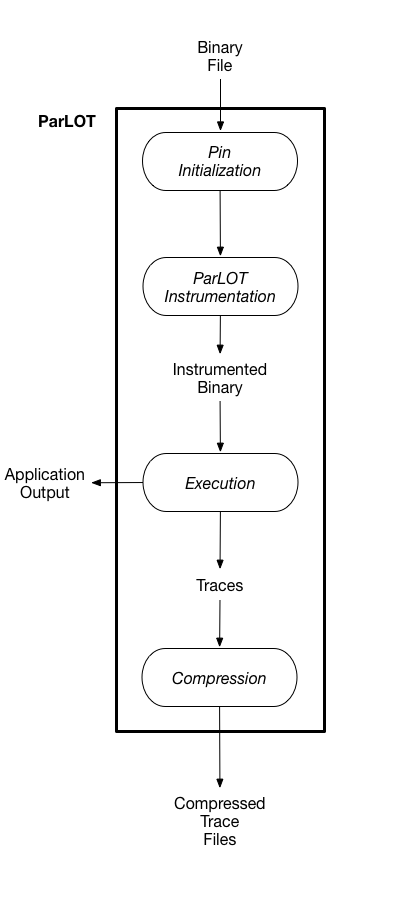
\includegraphics[width=2in]{overview.png}
\caption{Overview of \parlot}
\label{overview}
\end{figure}


\subsection{Evaluation of our Compression Scheme}

We conducted a preliminary evaluation of our compression
scheme by implementing a tracer in PIN that
records a unique 16-bit identifier for every function call and
return. 
%
Tracing just this small amount of information when running the
Mantevo miniapps~\cite{mantevo} on Stampede results in about 2 MB/s of
data per core on average. Extrapolating this value to all 102,400
cores of Stampede (not counting accelerators) yields 205 GB/s of trace
data, which exceeds the Lustre filesystem's write performance of 150
GB/s! 
%
Adding a simple compression algorithm that CRUSHER created 
reduces the emitted trace data by a factor of 100 on average,
a ratio that is very stable w.r.t scaling, making it possible to trace
full-scale programs while leaving over 98\% of the I/O bandwidth to
the application. 
%
This level of compression efficiency is also apparent in the 
results that we will present beginning \S\ref{sec:results}.

%--end




\section{Background and Related Work}
\label{sec:bgreltool}
\subsection{Binary Instrumentation}
Recording a log of events during the execution of an application is essential for better understanding the program behavior and, in case of a failure, to locate the problem. Recording this type of information requires instrumentation of the program either at the source-code or the binary-code level. Instrumenting the source code by adding extra statements to collect the desired information is easy for developers. However, doing so modifies the code and requires recompilation, often involving multiple different tools and complex hierarchies of makefiles, which can make this approach cumbersome and frustrating for users. Instrumenting an executable at the binary level using a tool is much easier, faster, and less error prone for most users. Moreover, binary instrumentation is language independent, portable to any system that has the appropriate instrumentation tool installed, and provides machine-level insight into the behavior of the application.

Executables can be instrumented \textit{statically}, where the additional code is inserted into the binary before execution, which results in a persistent modified executable, or \textit{dynamically}, where the modification of the executable is not permanent. In dynamic binary instrumentation, code can be discovered at runtime, making it possible to handle dynamically-generated and self-modifying code. Furthermore, it may be feasible to attach the instrumentation to a running process, which is particularly useful for long-running applications.

Many different tools for investigating application behavior have been designed on top of such Dynamic Binary Instrumentation (DBI) frameworks. For instance, Dyninst~\cite{dyninst} provides a dynamic instrumentation API that gives developers the ability to measure various performance aspects. It is used in tools like Open-SpeedShop~\cite{openss} and TAU~\cite{tau} as well as correctness debuggers like STAT~\cite{stat}. Moreover, VampirTrace~\cite{vampirt} uses it to provide a library for collecting program execution logs. 

Valgrind~\cite{valgrind} is a shadow-value DBI framework that keeps a copy of every register and memory location. It provides developers with the ability to instrument system calls and instructions. Error detectors such as Memcheck~\cite{memcheck} and call-graph generators like \callgrind~\cite{callgrind} are built upon Valgrind.\footnote{Given the absence of tools similar to \parlot, we employ \callgrind
 as a ``close-enough'' tool in our comparisons elaborated in \S\ref{sec:tracing-tools}.
 In this capacity, \callgrind is similar to \parlotm, a variant of \parlot that only collects
 traces from the {\tt main} function. We perform such comparison to have an idea of how we fare
 with respect to one other tool. \S\ref{sec:results} separately
 presents a ``self assessment'' of \parlot.}

 
%


We designed \parlot on top of \pin~\cite{pin}, a DBI framework for the IA-32, x86-64, and MIC instruction-set architectures for creating dynamic program analysis tools.\hl{ There is also version of PIN available for ARM architecture}\cite{pinarm}. \parlot mutates \pin to track the function call stack and to trace the entry (call) and exit (return) of every executed function. \hl{However, the mechanism of our tracing and compressing approaches can be built on top of other instrumentation tools and not restricted to pin. For example, PMaC }\cite{pmac} \hl{ is a DBI tool available for PowerPC/AIX architecture and ParLOT can be built on top of that.}


\subsection{Efficient Tracing for Debugging}
When dealing with large-scale parallel programs, any attempt to capture reasonably frequent events will result in a vast amount of data. Moreover, transferring and storing the data will incur significant overhead. For example, collecting just one byte of information per executed instruction yields on the order of a gigabyte of data per second on a single high-end core. Storing the resulting multi-gigabyte traces from many cores can be a challenge, even on today's large hard disks.

Hence, we need a way to decrease the space and runtime overhead. Compression can encode the generated data using a smaller number of bits, help
reduce the amount of data movement across the memory hierarchy, and
reduce storage and network demands.
%
Although the encoded data will later have to be decoded for analysis, compressing them during tracing enables the collection of much more information.

The use of compression by itself is not new.
Various performance evaluation tools~\cite{tau,scorep,eventflowgraph} 
already employ compression during the collection
of performance analysis data.
%
Tools such as ScalaTrace~\cite{scalatrace}
are also known to exploit
the repetitive nature of time-step simulations~\cite{freitag}. %Martin: unclear to me

\hl{
Many performance and debugging tools for HPC applications} \cite{stat,taumrnet}\hl{ had been built on top of MRNet}\cite{mrnet}\hl{ as an efficient overlay network for customizable data collection. MRNet overcomes the challenge of managing massive amount of trace data by distributing the workload of data collection, transfer and analysis among processes on a tree-based network. In contrast, ParLOT is taking advantage of data compression to increase efficiency and vastly reduce required bandwidth for data transfer. }

The novelty offered by \parlot lies in the combination of compression
speed, efficacy, and low timing jitter
made possible by its {\em incremental}
compression algorithm, which is
described in \S\ref{sec:design}.
%
It immediately compresses all traced information while the application is running, that is, \parlot never even records the uncompressed trace in memory. 
%
Typically, just a few kilobytes of data need to be written out per thread and per second, thus requiring only a small fraction of the available disk or network bandwidth. 
%
The traces are decompressed later at no additional cost to the execution of the application. 
%
From the decompressed full function-call trace, the complete call-graph, 
call-frequency, and caller-callee information can be extracted. 
%
This can be done at the granularity of a thread, a group of threads, or the whole application.
%
We now elaborate on the design of \parlot that makes
these innovations possible.
%--










\section{Case Studies}
\label{sec:case}
\subsubsection{Case Study: ILCS}
ILCS \cite{ilcs}
\subsubsection{Case Study: MFEM}


    
\section{Discussion and Future Work}
\label{sec:discussion}


 
%--end



\bibliographystyle{ACM-Reference-Format}
\bibliography{bibs}


\end{document}
